\documentclass[a4paper,12pt]{article}
\usepackage{amsfonts}
\usepackage{amsthm}
\usepackage{amsmath}
\usepackage{listings}
\usepackage{xcolor}
\usepackage[margin=1.0in]{geometry}
\usepackage{setspace}
\usepackage{lipsum}
\usepackage{etoolbox}
\usepackage{float}
\usepackage{tikz}
\usepackage{fourier}
\usepackage{subcaption}
\AtBeginEnvironment{quote}{\singlespace\vspace{-\topsep}\small}
\AtEndEnvironment{quote}{\vspace{-\topsep}\endsinglespace}
\definecolor{lightergray}{gray}{0.95}

\newcommand{\tabitem}{~~\llap{\textbullet}~~}

\theoremstyle{remark}
\newtheorem*{remark}{Remark}

\lstloadlanguages{Haskell}
\lstnewenvironment{code}
    {\lstset{}%
      \csname lst@SetFirstLabel\endcsname}
    {\csname lst@SaveFirstLabel\endcsname}
    \lstset{
      basicstyle=\small\ttfamily,
      flexiblecolumns=false,
      basewidth={0.5em,0.45em},
      moredelim=[is][\underbar]{_}{_},
      mathescape=true, % needed for subscripts
      keepspaces=true,
      literate={+}{{$+$}}1 {/}{{$/$}}1 {*}{{$*$}}1 {=}{{$=$}}1
               {>}{{$>$}}1 {<}{{$<$}}1 {\\}{{$\lambda$}}1
               {\\\\}{{\char`\\\char`\\}}1
               {->}{{$\rightarrow$}}2 {>=}{{$\geq$}}2 {<-}{{$\leftarrow$}}2
               {<=}{{$\leq$}}2 {=>}{{$\Rightarrow$}}2
               {\ .}{{$\circ$}}2 {\ .\ }{{$\circ$}}2
               {>>}{{>>}}2 {>>=}{{>>=}}2
               {|}{{$\mid$}}1
               {<*}{$\langle *$}{1}
               {*>}{$* \rangle$}{1}
               {<s}{$\langle \$$}{1}
               {s>}{$\$ \rangle$}{1}
               {<~}{$\langle \sim$}{1}
               {~>}{$\sim \rangle$}{1}
               {<*>}{$\langle * \rangle$}{2}
               {<|>}{$\langle | \rangle$}{2}
               {<s>}{$\langle \$ \rangle$}{2} % workaround to allow mathescape
               {<:>}{$\langle : \rangle$}{2}
               {<*>}{$\langle * \rangle$}{2}
               {<~>}{$\langle \sim \rangle$}{2}
               {\\/}{$\nabla$}{2}
               {empty_string}{$\varepsilon$}{1}
    }




\begin{document}
	\title{Language Engineering (TB1)}
  \author{Taken by Joseph MacManus\\
          on a course given by Dr Nicolas Wu (2018)}
	\maketitle
	\pagenumbering{roman}
	\tableofcontents
	\newpage
	\pagenumbering{arabic}

  \sloppy
  \setlength{\parindent}{0em}
  \setlength{\parskip}{1em}

  \section{DSLs and Catamorphisms}

  \subsection{Domain-Specific Languages}

  A programming language consists of three main components:
  \begin{itemize}
    \item Syntax - the shape of grammer / words / vocab.
    \item Semantics - the meaning; a function from syntax to some domain.
    \item Pragmatics - The purpose of a language.
  \end{itemize}

  A domain-specific language (DSL) is a language that has been crafted with a
  specific purpose in mind. These are not necessarily Turing-complete.
  Some DSLs come equipped with all the features of general purpose languages:
  \begin{itemize}
    \item Parser
    \item Syntax highlighting
    \item IDE
    \item Compiler
    \item Documentation
  \end{itemize}

  and so on. An embedded DSL (EDSL) is defined within another host language. The
  advantage is that there is less work to perfom, but this is at the cost of
  restricted flexibility. An EDSL can be either a \textit{deep} or \textit{shallow} embedding. A
  deep embedding is where the syntax is given by concrete datatypes, and the semantics given by
  evaluation. A shallow embedding has syntax borrowed directly from it's host language,
  and semantics is directly given.

  For example, consider:
  \["3+5" \textrm{\ \ in a string.}\]
  \[ \llbracket 3+5\rrbracket \textrm{ \ :: \ Int} \]

  Where $\llbracket \rrbracket$ are denotational brackets. We use them to ascribe a semantics.

  \[ \llbracket 3+5\rrbracket = \llbracket 3\rrbracket + \llbracket 5 \rrbracket = 3+5 = 8 \]

  We can model this using a deep embedding in Haskell with the following code:

  \begin{lstlisting}
        data Expr = Var Int
                  | Add Expr Expr

        eval :: Expr -> Int
        eval (Var n) = n
        eval (Add x y) = (eval x) + (eval y)  \end{lstlisting}

  So instead of $\llbracket 3 + 5 \rrbracket$, we can now write
  \lstinline{eval (Add (Var 3) (Var 5))}.

  The shallow embedding is given directly by functions: (We will redefine
  \lstinline{Expr} here)

  \begin{lstlisting}
        type Expr = Int

        var :: Int -> Expr
        var n = n

        add :: Expr -> Expr -> Expr
        add x y = x + y  \end{lstlisting}

  Our example is now written as:

  \begin{lstlisting}
        add (var 3) (var 5)  \end{lstlisting}

\begin{remark}
  What is a compiler, then? A compiler is code that transforms a language to a
  target language through some intermediate representation.

  \begin{figure}[H]
    \centering
    \fbox{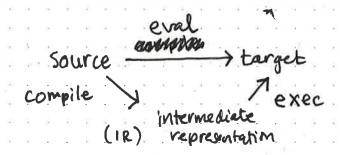
\includegraphics[width=220pt]{images/2-1.png}}
    % \caption{ CAPTION }
  \end{figure}

  Typical examples of this diagram include the C compiler gcc, which takes a C
  source file and compiles this to assembly. That assembly is then executed in
  the terminal. Javascript tends to ignore the compile stage since it is an interpreted
  language. The web browser performs eval, which turns JS into rendered output.
  Haskell has two modes, when using GHC, it compiles .hs files into assembly,
  which can then be executed in the terminal. However, when using GHCi, it takes
  source code and interprets it directly by evaluating in the terminal.

\end{remark}

  \subsection{Case Study: Circuit Language}

  We will study a particular example of a DSL, and the different ways to embed it
  in Haskell. The circuit language is a DSL for describing circuits. It consists of several
  operations. Rather than define each operation formally, we shall give the type of each
  operation and an example of what it does.

  % TODO circuit language

  \begin{itemize}
    \item \lstinline{identity :: Int -> Circuit}

    \begin{figure}[H]
      \centering
      \fbox{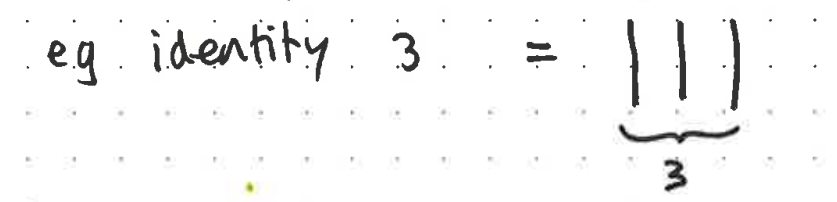
\includegraphics[width=180pt]{images/2-2.png}}
      % \caption{ CAPTION }
    \end{figure}

    \item \lstinline{beside :: Circuit -> Circuit -> Circuit}

    \begin{figure}[H]
      \centering
      \fbox{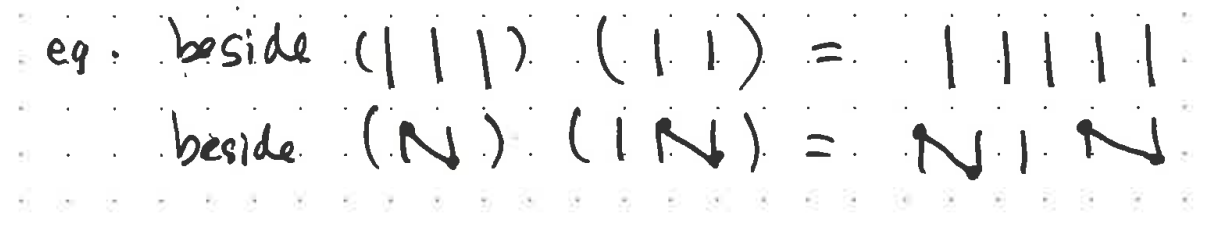
\includegraphics[width=180pt]{images/2-2-1.png}}
      % \caption{ CAPTION }
    \end{figure}

    \item \lstinline{above :: Circuit -> Circuit -> Circuit}

    \begin{figure}[H]
      \centering
      \fbox{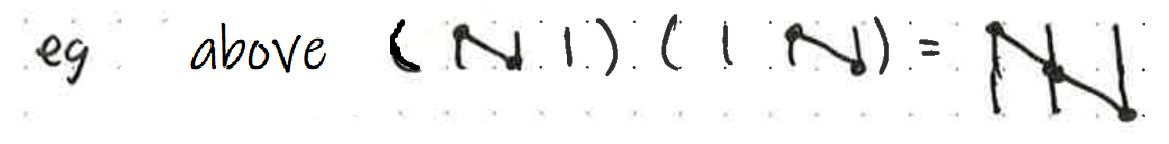
\includegraphics[width=180pt]{images/2-3.png}}
      % \caption{ CAPTION }
    \end{figure}

    \item \lstinline{fan :: Int -> Circuit}

    \begin{figure}[H]
      \centering
      \fbox{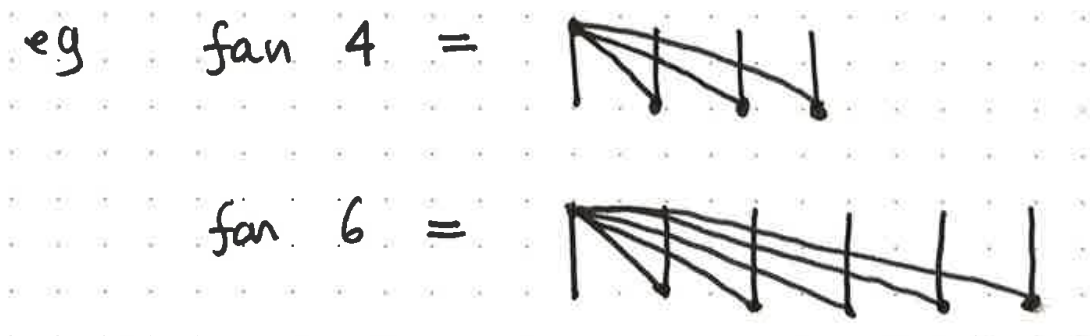
\includegraphics[width=180pt]{images/2-3-1.png}}
      % \caption{ CAPTION }
    \end{figure}

    \item \lstinline{stretch :: [Int] -> Circuit -> Circuit}

    \begin{figure}[H]
      \centering
      \fbox{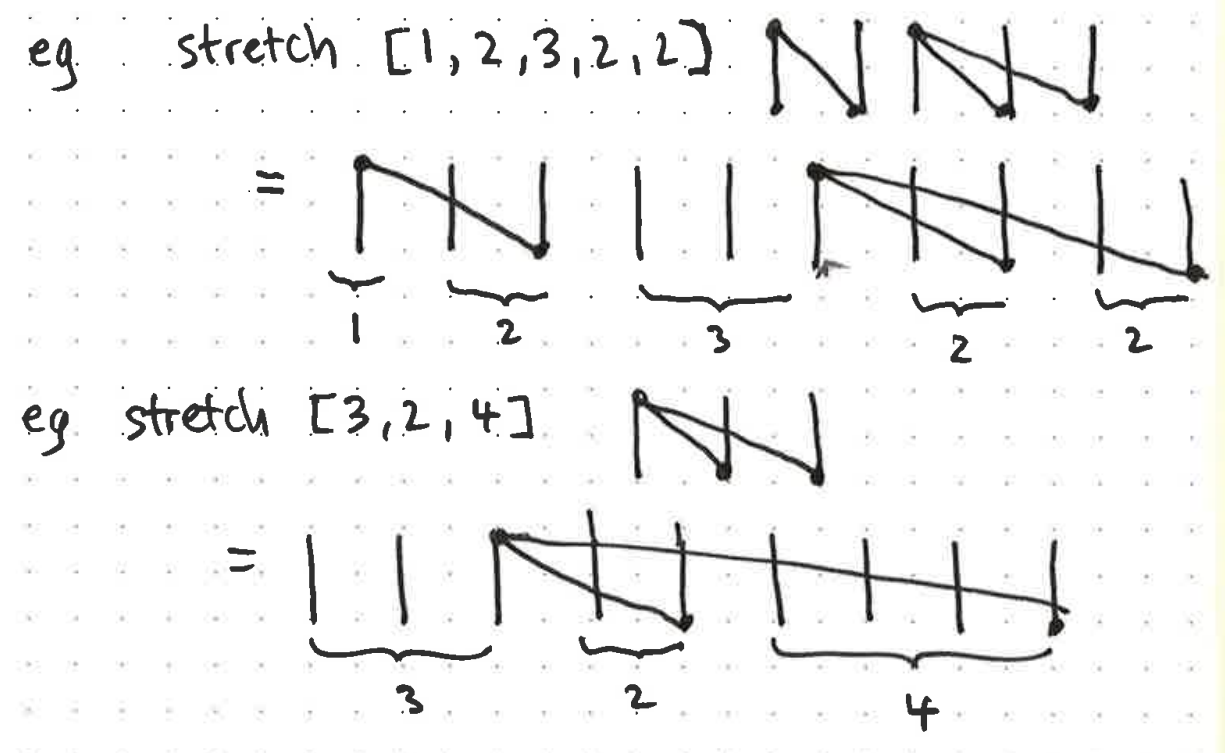
\includegraphics[width=180pt]{images/2-3-2.png}}
      % \caption{ CAPTION }
    \end{figure}

  \end{itemize}

  This language is used to describe how circuits work, information starts at the
  top of each line and travels downwards. Information is combined by joining lines,
  and applying the associative operation of our choosing:

  \begin{figure}[H]
    \centering
    \fbox{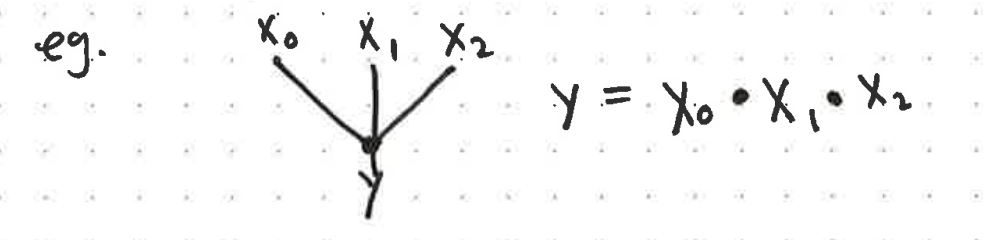
\includegraphics[width=180pt]{images/2-4.png}}
    % \caption{ CAPTION }
  \end{figure}

  And information is duplicated when lines seperate:

  \begin{figure}[H]
    \centering
    \fbox{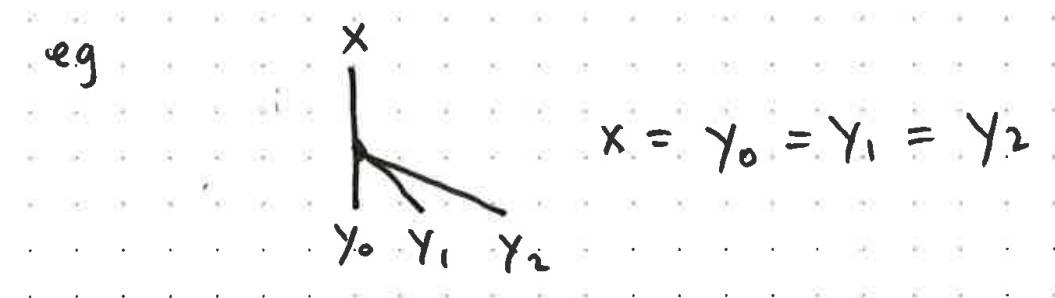
\includegraphics[width=180pt]{images/2-4-1.png}}
    % \caption{ CAPTION }
  \end{figure}

  There are many different ways of interpeting this circuit language. For example,
  we may want to simply find the width or height of a circuit, or perhaps we will
  evaluate the output of a circuit given an input and the node operation. We start
  with a deep embedding. This is achieved in two steps:
  \begin{enumerate}
    \item Create a data structure for the abstract syntax.
    \item Define a semantics with an evaluation function.
  \end{enumerate}

  The first step isn't too hard, we simply get:

  \begin{lstlisting}
      data Circuit = Identity Int
                   | Beside Circuit Circuit
                   | Above Circuit Circuit
                   | Fan Int
                   | Stretch [Int] Circuit  \end{lstlisting}

  Let's interpet the circuit language by stipulating that the semantics of a term is
  the width of the circuit generated. We will define a semantics with a function \lstinline{width}.

  \begin{lstlisting}
      type Width = Int

      width :: Circuit -> Width
      width (Identity n) = n
      width (Beside $c_1$ $c_2$) = (width $c_1$) + (width $c_2$)
      width (Above $c_1$ $c_2$) = width $c_1$
      width (Fan n) = n
      width (Stretch ws c) = sum ws  \end{lstlisting}

  We can have multiple semantics easily by supplying more evaluation functions. For
  instance, the height of the circuit is:

  \begin{lstlisting}
      type Height = Int

      height :: Circuit -> Height
      height (Identity n) = 1
      $\dots$
      height (Above $c_1$ $c_2$) = height $c_1$ + height $c_2$  \end{lstlisting}

  Sometimes the semantics are interwined in a dependent way. For instance, calculating
  if a circuit is well connected requires us to calculate the width even though all
  we are interested in is one bool.

  \begin{lstlisting}
      type Connected = Bool

      connected :: Circuit -> Connected
      connected (Identity n) = True
      connected (Beside $c_1$ $c_2$) = connected $c_1$ && connected $c_2$
      connected (Above $c_1$ $c_2$) = connected $c_1$ && connected $c_2$
                                && width $c_2$ == width $c_2$
      connected (Fan n) = True
      connected (Stretch ws c) = connected c && width c == length ws
                                && (not . (elem 0)) ws  \end{lstlisting}

  In a shallow embedding we simply have to give a semantics in terms of the operations
  directly.

  \begin{lstlisting}
      type Width = Int

      type Circuit = Width

      identity :: Int -> Circuit
      identity n = n

      beside :: Circuit -> Circuit -> Circuit
      beside $c_1$ $c_2$ = $c_1$ + $c_2$

      above :: Circuit -> Circuit -> Circuit
      above $c_1$ $c_2$ = $c_1$

      fan :: Int -> Circuit
      fan n = n

      stretch :: [Int] -> Circuit -> Circuit
      stretch ws c = sum ws  \end{lstlisting}

  Shallow is problemaic because it is hard to add a different semantics. In order
  to do so we must redefine Circuit, but this might break any code that depends on
  the old definition. Additionally, a dependent semantics requires all of the interpretations
  to be considered at once. This is not compositioned. However, in a shallow semantics
  it is easy to extend the language with new operations,
  since this involves adding new functions: nothing breaks. With a deep embedding a
  new constructor must be added, so all semtantics must be extended accordingly.

  \textit{Is it possible to extend the syntax and semtnaics of a language in a
  modular fashion?} This is known as \textit{The Expression Problem}. For instance,
  consider the data type \lstinline{Expr} from before:

  \begin{lstlisting}
      data Expr =val Int | Add Expr Expr  \end{lstlisting}

  Here we want to extend the syntax by adding a new operation for multiplication,
  but we do not want to modify any existing code. I.e. we cannot simply add a new
  \lstinline{Mul} constructor. Similarly, consider the semantics:

  \begin{lstlisting}
      eval :: Expr -> Int  \end{lstlisting}

  Again, we want to extend the semantics without modifying the code. (Though in this
  case adding semantics is easy as we simply write another function of type \lstinline{Expr -> b}).
  To solve the expression problem, we will study a generalisation of folds called
  a \textit{catamorphism}. We do this because folds are a way of reducing data structures in a
  composable way, and syntax trees are just data structures.

  \subsection{Catamorphisms}

  Consider the fold for a list:

  \begin{lstlisting}
      data [a] = []
               | a : [a]

      foldr :: b -> (a -> b -> b) -> [a] -> b
      foldr k f [] = k
      foldr k f (x:xs) = f x (foldr k f xs)  \end{lstlisting}

  How do we generalise this? Our first step is to deconstruct the type of lists to expose its generic structure.
  The defintion of lists is the same as the following, when we remove the syntactic sugar.

  \begin{lstlisting}
      data List a = Empty
                  | Cons a (List a)  \end{lstlisting}

  We remove recursion from this data type, and mark it was a parameter \lstinline{k},
  for \textit{k}ontinuation.

  \begin{lstlisting}
      data _List_ a k = _Empty_
                     | _Cons_ a k  \end{lstlisting}

  Next, we make the recursive paramter something we can change programatically by
  giving a Functor instance to \lstinline{_List_} a

  \begin{lstlisting}
      instance Functor (_List_ a) where
          fmap :: (x -> y) -> _List_ a x -> _List_ a y
          fmap f _Empty_ = _Empty_
          fmap (_Cons_ a x) = _Cons_ a (f x)  \end{lstlisting}

  We now need to derive a type that gives us the fixed point of data. This is defined
  as follows:

  \begin{lstlisting}
      data Fix f = In (f (Fix f))  \end{lstlisting}

  This datatype allows us to generalise all recursive data types (except mutually
  recursive ones). For example, instead of \lstinline{List a}, we can write \lstinline{Fix (_List_ a)}. To
  demonstrate this, we show that \lstinline{List a} and \lstinline{Fix (_List_ a)} are isomorphic.

  \begin{lstlisting}
      toList :: Fix (_List_ a) -> List a
      fromList :: List a -> Fix (_List_ a)  \end{lstlisting}

  We say that \lstinline{List a} and \lstinline{_List_ a} are isomorphic when composing the above functions
  in any order yields the identity. Let's define these functions.

  \begin{lstlisting}
      fromList :: List a -> Fix (_List_ a)
      fromList Empty = In _Empty_  \end{lstlisting}

  Some examples of values of type \lstinline{Fix (_List_ a)} are:

  \begin{lstlisting}
      In _Empty_ :: Fix (_List_ a)  \end{lstlisting}

  (Note that the type of \lstinline{In} is \lstinline{In :: f (Fix f) -> Fix f}
  so the example above is where \lstinline{f} is \lstinline{_List_ a}.)

  \begin{lstlisting}
      In (_Cons_ 5 (In _Empty_))  \end{lstlisting}

  and for two elements we have

  \begin{lstlisting}
      In (_Cons_ 6 (In (_Cons_ 7 (In _Empty_))))  \end{lstlisting}

  So now we have enough to finish a definition of \lstinline{fromList}.

  \begin{lstlisting}
      fromList :: List a -> Fix (_List_ a)
      fromList Empty = In EmmptyF
      fromList (Cons x xs) = In (_Cons_ x (fromList xs))  \end{lstlisting}

  We are now ready to generise fold to be a catamorphism. Consider functions of the form
  \lstinline{_List_ a b -> b}:

  \begin{lstlisting}
      h :: _List_ a b -> b
      h _Empty_ = k
      h (_Cons_ a y) = f a y
          where
              k :: b
              f :: a -> b -> b  \end{lstlisting}

  Functions of that type correspond to replacing the constructors of \lstinline{_List_ a} with functions \lstinline{k}
  and \lstinline{f} just like in \lstinline{foldr}. A catamorphism arises from this diagram:

  \begin{figure}[H]
    \centering
    \fbox{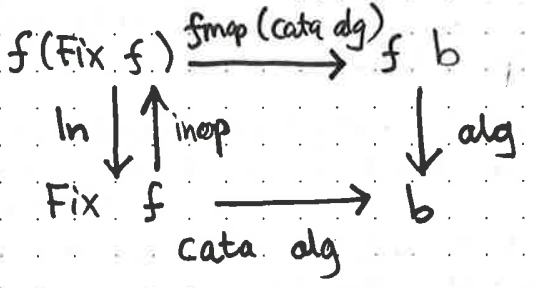
\includegraphics[width=180pt]{images/5-2.png}}
    % \caption{ CAPTION }
  \end{figure}

  The function \lstinline{inop} is the opposite of \lstinline{In}. We define it by the following:

  \begin{lstlisting}
      inop :: Fix f -> f (Fix f)
      inop (In x) = x  \end{lstlisting}

  So finally we can write the function cata by chasing the arrows of this square:

  \begin{lstlisting}
      cata :: Functor f => (f b -> b) -> Fix f -> b
      cata alg x (alg . fmap (cata alg) . inop) x  \end{lstlisting}

  An alternative and equivalent definition is:

  \begin{lstlisting}
      cata alg (In x) = alg (fmap (cata alg) x)  \end{lstlisting}

  To use this, we only need to supply the \lstinline{alg}. We will define the function \lstinline{toList}
  using a \lstinline{cata}:

  \begin{lstlisting}
      toList :: Fix (_List_ a) -> List a
      toList = cata alg
          where
              alg :: _List_ a (List a) -> List a
              alg _Empty_ = Empty
              alg _Cons_ x xs = Cons x xs  \end{lstlisting}

  or, equivalently

  \begin{lstlisting}
      toList' :: Fix (_List_ a) -> [a]
      toList' cata alg
          where
              alg :: _List_ a [a] -> [a]
              alg _Empty_ = []
              alg _Cons_ x xs = x : xs  \end{lstlisting}

  We can also define a function that returns the length of a \lstinline{Fix (_List_ a)}.

  \begin{lstlisting}
      length :: Fix (_List_ a) -> Int
      length :: cata alg
          where
              alg :: _List_ a Int -> Int
              alg _Empty_ = 0
              alg (_Cons_ x y) = y + 1  \end{lstlisting}

  Here is an example of evaluation.

  \begin{lstlisting}
      length (In(_Cons_ 7 (In (_Cons_ 9 (In _Empty_)))))
    = {length}
      cata alg (In (_Cons_ 7 (In (_Cons_ 9 (In _Empty_)))))
    = {cata}
      alg (fmap (cata alg) (_Cons_ 7 (In $\ldots$)))
    = {fmap}
      alg (_Cons_ 7 (cata alg (In (_Cons_ 9 (In _Empty_)))))
    = {alg}
      1 + cata alg (In (_Cons_ 9 (In _Empty_)))
    = {cata}
      1 + alg (fmap (cata alg) (_Cons_ 9 (In Empty)))
    = {fmap}
      1 + alg (_Cons_ 9 (cata alg (In _Empty_)))
    = {alg}
      1 + 1 + cata alg (In _Empty_)
    = {cata}
      1 + 1 + alg (fmap (cata alg) _Empty_)
    = {fmap}
      1 + 1 + alg _Empty_
    = {alg}
      1 + 1 + 0
    = {(+)}
      2  \end{lstlisting}

  Now another exmaple, of summing a list.

  \begin{lstlisting}
      sum :: Fix (_List_ Int) -> Int
      sum = cata alg
          where
              alg :: _List_ Int Int -> Int
              alg _Empty_ = 0
              alg (Cons x y) = x + y  \end{lstlisting}

  \subsection{Case Study: Peano Numbers}

  A Peano number is either zero, or a successor of another Peano number.

  \begin{lstlisting}
      data Peano = z
                 | S Peano  \end{lstlisting}

  So the number 3 is written $S(S(S (0)))$. Our goal is to create a
  modular DSL which models Peano numbers, a fashion similar to above.
  Step 1: make a signature functor for \lstinline{Peano}.

  \begin{lstlisting}
      data _Peano_ k = z
                   | S k  \end{lstlisting}

  Step 2: Define a functor instance for \lstinline{_Peano_}.

  \begin{lstlisting}
      instance Functor _Peano_ where
          fmap :: (a -> b) -> _Peano_ a -> _Peano_ b
          fmap f z = z
          fmap f (S x) = S (f x)  \end{lstlisting}

  Step 3: Write functions using \lstinline{cata}.

  \begin{lstlisting}
      toInt :: Fix _Peano_ -> Int
      toInt = cata alg where
          alg :: _Peano_ Int -> Int
          alg z = 0
          alg (S x) = x + 1  \end{lstlisting}

  Now we can define a doubling function.

  \begin{lstlisting}
      double :: Fix _Peano_ -> Fix _Peano_
      double = cata alg  where
          alg :: _Peano_ -> Fix _Peano_
          alg z = In z
          alg (S x) = In( S (InS ( x )))  \end{lstlisting}

  \subsection{Composing Languages}

  Previously, we looked at the following data type as the language for addition.

  \begin{lstlisting}
      data Expr = Val Int
                | Add Expr Expr  \end{lstlisting}

  We then learnt to extract the signature functor for this by locating recursive calls:

  \begin{lstlisting}
      data _Expr_ k = _Val_ Int
                   | _Add_ k k  \end{lstlisting}

  The \lstinline{Fix _Expr_} datatype is essentially \lstinline{Expr}. Suppose we want to add multiplication
  to this language. We need a way to extend \lstinline{_Expr_} with more constructors. This is
  achieved by the coproduct of functors. The coproduct functor is defined as:

  \begin{lstlisting}
      data (f :+: g) a = L(f a)
                       | R(g a)  \end{lstlisting}

  This takes two functors and makes the functor \lstinline{(f:+:g)}. It introduces these
  constructors:

  \begin{lstlisting}
      L :: f a -> (f:+:g) a
      R :: g a -> (f:+:g) a  \end{lstlisting}

  The functor instance is defined as follows

  \begin{lstlisting}
      instance (Functor f, Functor g) => Functor (f:+:g) where
          fmap :: (a -> b) -> (f:+:g) a -> (f:+:g) b
          fmap f (L x) = L (fmap f x)
          fmap f (R y) = R (fmap f y)  \end{lstlisting}

  Now we are ready to define the signature functor for multiplication:

  \begin{lstlisting}
      data _Mul_ k = _Mul_ k k  \end{lstlisting}

  This is the datatype constructor:

  \begin{lstlisting}
      _Mul_ :: k -> k -> _Mul_ k  \end{lstlisting}

  We define its functor instance:

  \begin{lstlisting}
      instance Functor _Mul_ where
          fmap f (Mul x y) = _Mul_ (f x) (f y)  \end{lstlisting}

  Finally, we can put the \lstinline{_Expr_} and \lstinline{_Mul_} languages together, to have a language with
  both addition and multiplication.

  \begin{lstlisting}
      Fix (_Expr_ :+: _Mul_)  \end{lstlisting}

  This is essentially the same as describing the following datatype, but in a
  compositional way:

  \begin{lstlisting}
      data Expr' = Val' Int
                 | Add' Expr' Expr'
                 | Mul' Expr' Expr'  \end{lstlisting}

  For practical purposes, we do not work with \lstinline{Expr'} but with \lstinline{Fix (_Expr_ :+: _Mul_)}.
  We need to write algebras\footnote{An \textit{algebra} is any function of type \lstinline{f a -> a},
  where \lstinline{f} is a functor.} of the form:

  \begin{lstlisting}
      Expr :+: Mul b -> b  \end{lstlisting}

  to reduce a \lstinline{Fix (_Expr_ :+: _Mul_)} type to  \lstinline{b}. To do this in a composotional way,
  we define a way of combining \lstinline{_Expr_} algebras and \lstinline{_Mul_} algebras. We call this the
  junction of algebras:

  \begin{lstlisting}
      (\/) :: (f a -> a) -> (g a -> a) -> ((f:+:g) a -> a)
      (falg \/ galg) (L x) = falg x
      (falg \/ galg) (R y) = galg y  \end{lstlisting}

  So now, we can give a semantics to the language \lstinline{Fix (Expr:+:Mul)} by defining algebras.

  \begin{lstlisting}
      add :: _Expr_ Int -> Int
      add (_Val_ x) = x
      add (_Add_ x y) = x + y

      mul :: _Mul_ Int -> Int
      mul (_Mul_ x y) = x * y  \end{lstlisting}

  To evaluate, we write:

  \begin{lstlisting}
      eval :: Fix (_Expr_ :+: _Mul_) -> Int
      eval = cata (add \/ mul)  \end{lstlisting}

  And thus, we have solved the expression problem. In fact, we can decompose the \lstinline{_Expr_}
  into constituent parts:

  \begin{lstlisting}
      data _Val_ k = _Val_ Int

      data _Add_ k = _Add_ k k  \end{lstlisting}

  After defining functor instances, we can define functor instances for:

  \begin{lstlisting}
      Fix (_Val_ :+: _Add_ :+: _Int_)  \end{lstlisting}

  \section{Grammars and Parsers}

  \subsection{BNF: Baccus-Naur Form}

  BNF is a language used to express the shape of grammars. It was invented in around
  1958 for the expression of the Algol programming language. A BNF statement is made
  up of:

  \begin{itemize}
    \item \lstinline{empty_string} represents empty strings.
    \item \lstinline{<n>} represents a non-terminal.
    \item \lstinline{"x"} represents a terminal.
    \item \lstinline{p|q} represents a choice between \lstinline{p} and \lstinline{q}.
  \end{itemize}

  An example of BNF is the following:

  \begin{lstlisting}
      <digit> ::= "0" | "1" | "2" | $\ldots$ | "8" | "9"
          // ::= signifies defintion.  \end{lstlisting}

  We can aproximate numbers by this:

  \begin{lstlisting}
      <num> ::= <digit>
             |  <digit><num>  \end{lstlisting}

  The core language of BNF is usually extended with some constructs:

  \begin{lstlisting}
      [ e ]  // optional e
      ( e )  // grouping e
        e*   // 0 or more repetitions of e
        e+   // 1 or more repetitions of e  \end{lstlisting}

For a more complex example, consider expressions:

\begin{lstlisting}
    <expr> ::= <num>
            |  <num> "+" <expr>  \end{lstlisting}

This corresponds to the following type:

\begin{lstlisting}
    data Expr = Val Num
              | Add Num Expr  \end{lstlisting}

In principle, we do the same to convert \lstinline{<num>} into a Num datatype. However,
we will approximate this by the type Int.

\begin{lstlisting}
    type Num = Int  \end{lstlisting}

Grammars can sometimes be ambiguous, a single string can be accepted by the grammar
in multiple ways:

\begin{lstlisting}
    <expr> ::= <num>
            |  <expr> "+" <expr>  \end{lstlisting}

The problem here is also that \lstinline{<expr>} is left-recursive: there is a branch which
has an \lstinline{<expr>} before any terminal. This causes problems in recursive descent parsers,
which we will study later. The solution is to refactor the grammar.

\subsection{Paull's Modified Algorithm}

We can remove recursion as follows. Suppose we have the following grammar:

\begin{lstlisting}
    A ::= A $\alpha_1$ | $\cdots$ | A $\alpha_n$ | $\beta_1$ | $\cdots$ | $\beta_m$  \end{lstlisting}

To apply the algorithm, we rewrite the term above to be the following:

\begin{lstlisting}
    A  ::= $\beta_1$ A' | $\cdots$ | $\beta_m$ A'
    A' ::= $\alpha_1$ A' | $\cdots$ | $\alpha_n$ A' | empty_string  \end{lstlisting}

In practive here is how we convert the following:

\begin{lstlisting}
    <expr> ::= <num>
            |  <expr> "+" <expr>

    // becomes

    <expr> ::= <num> <expr'>
    <expr'> ::= "+" <expr> <expr'> | empty_string  \end{lstlisting}

\subsection{Parsers}

A parser is a function that takes in a list of characters, and returns an item that
was parsed, along with the unconsumed string. We can define it by:

\begin{lstlisting}
    newtype Parser a = Parser (String -> [(a, String)])  \end{lstlisting}

We can use a parser by defining a function, parse.

\begin{lstlisting}
    parse :: Parser a -> String -> [(a, String)]
    parse (Parser px) = px

    (px :: String -> [(a, String)])  \end{lstlisting}

Some very simple examples of parsers include the \lstinline{fail} parser which always fails,
the \lstinline{item} parser which knows how to process a single character, and the
\lstinline{look} parser, which allows one to look into the input stream without consuming anything.

\begin{lstlisting}
    fail :: Parser a
    fail = Parser ( \ ts -> [] )

    item :: Parser Char
    item :: Parser ( \ ts -> case ts of
                      [] -> []
                      (t:ts') -> [(t,ts')])

    look :: Parser String
    look = Parser (\ ts -> [(ts,ts)])

    -- e.g. parse (fail) "Hello" = []
    --      parse (item) "Hello" = [('H', "ello")]
    --      parse look "Hello" = [("Hello","Hello")]  \end{lstlisting}

Often we want to transform our parsers from producing values of one type to
another. For instance, we might transform a parser for a single \lstinline{Char} into producing
the corresponding \lstinline{Int}. This is achieved by giving a functor instance for parsers.
We can use this to define a \lstinline{Parser} for \lstinline{Int}s from our item parser (see the homework).

%% TODO add the Int parser example to here

\begin{lstlisting}
    instance Functor Parser where
      -- fmap :: (a -> b) -> Parser a -> Parser b
      fmap f (Parser px) =
              Parser ( \ts -> [(f x, ts') | (x, ts') <- px ts])

    (<s>) :: (a->b) -> Parser a -> Parser b
    f <s> px = fmap f px  \end{lstlisting}

The following variation is often useful:

\begin{lstlisting}
    (<s) :: a -> Parser b -> Parser a
    x <s py = fmap (const x) py  \end{lstlisting}

We can use this to build a function called \lstinline{skip} that parses input but outputs
nothing useful.

\begin{lstlisting}
    skip :: Parser a -> Parser ()
    skip px = () <s px  \end{lstlisting}

Now we want to apply a function to the different outputs of parse:

\begin{figure}[H]
  \centering
  \fbox{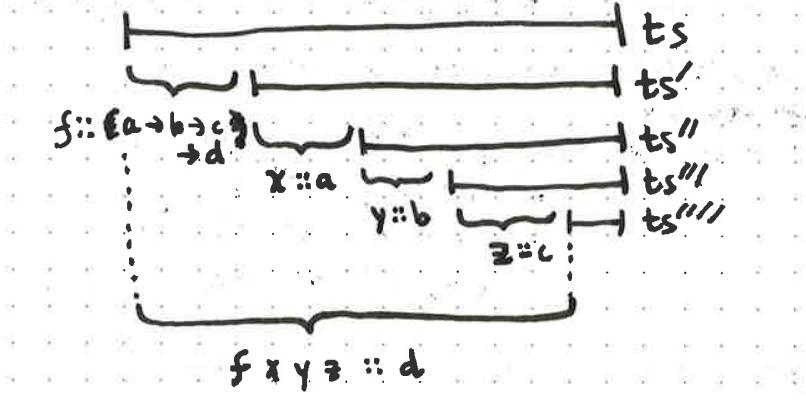
\includegraphics[width=180pt]{images/9-3.png}}
  % \caption{ CAPTION }
\end{figure}


To make something like this we use a combination of \lstinline{<*>} and \lstinline{<s>} like this:

\begin{lstlisting}
    pf <*> px <*> py <*> pz  \end{lstlisting}

This uses the \lstinline{(<*>)} operation, which we will define shortly. The applicative
introduces pure and \lstinline{(<*>)}.

\begin{lstlisting}
    class Functor f => Applicative f where
        pure :: a -> f a
        (<*>) :: f (a -> b) -> f a -> f b  \end{lstlisting}

These have the following definitions:

\begin{lstlisting}
    instance Application Parser where
        -- pure :: a Parser a
        pure x = Parser (\ts -> [(x,ts)])  \end{lstlisting}

The \lstinline{pure x} parser will not consume any input but always generates the value \lstinline{x}.

\begin{lstlisting}
    parse (pure 5) "hello" = [(5, "hello")]  \end{lstlisting}

Now we define \lstinline{(<*>)}, pronounced "ap", for apply.

\begin{lstlisting}
    -- (<*>) :: Parser (a -> b) -> Parser a -> Parser b
    Parser pf <*> Parser px = Parser ( \ts ->
                            [(f x, ts'')
                            | (f, ts')  <- pf ts
                            , (x, ts'') <- px ts' ])  \end{lstlisting}

\begin{figure}[H]
  \centering
  \fbox{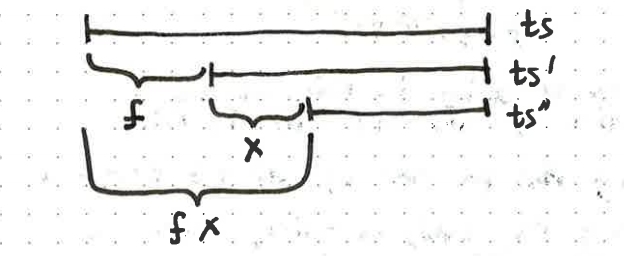
\includegraphics[width=180pt]{images/10-1.png}}
  % \caption{ CAPTION }
\end{figure}

The operation we defined first parses a function, then a value, and finally applies
the function to the value. Thos can be done the other way around too:

\begin{lstlisting}
    (<**>) :: Parser a -> Parser (a -> b) -> Parser b
    Parser px <**> Parser pf = Parser ( \ts ->
                             [ (f x, ts'')
                             | (x, ts')  <- px ts
                             , (f, ts'') <- pf ts' ])  \end{lstlisting}

\begin{figure}[H]
  \centering
  \fbox{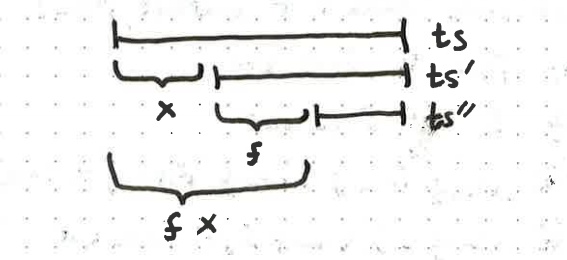
\includegraphics[width=180pt]{images/10-2.png}}
  % \caption{ CAPTION }
\end{figure}

Other derived operators are \lstinline{(<*)} and \lstinline{(*>)}, their types are:

\begin{lstlisting}
    (<*) :: Parser a -> Parser b -> Parser a
    (*>) :: Parser a -> Parser b -> Parser b  \end{lstlisting}

\subsection{Monoidal}

The \lstinline{Monoidal} class is equivalent to the \lstinline{Applicative} class:

\begin{lstlisting}
    class Monoidal f where
        unit :: f ()
        mult :: f a -> f b -> f (a,b)  \end{lstlisting}

For parsers, the \lstinline{monoidal} instance is defined as follows:

\begin{lstlisting}
    instance Monoidal Parser where
        -- unit :: Parser ()
        unit = Parser ( \ts -> [((), ts)])

        -- mult :: Parser a -> Parser b -> Parser (a,b)
        mult px py = Parser ( \ts ->
                   [ ((x,y), ts'')
                   | (x, ts')  <- px ts
                   , (y, ts'') <- py ts'])  \end{lstlisting}

\begin{figure}[H]
  \centering
  \fbox{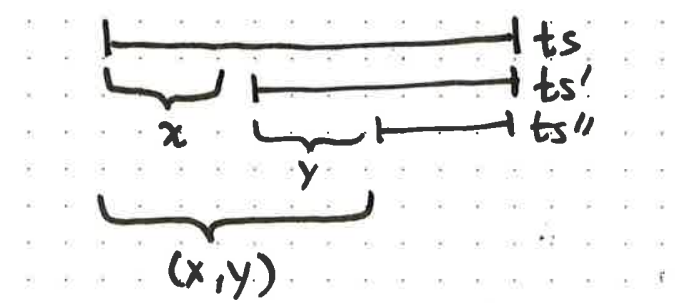
\includegraphics[width=180pt]{images/10-3.png}}
  % \caption{ CAPTION }
\end{figure}

It is useful to make \lstinline{mult} a binary operation, so we introduce one:

\begin{lstlisting}
    (<~>) :: Monoidal f => f a -> f b -> f (a,b)
    px <~> py = mult px py  \end{lstlisting}

We the derive these useful combinators:

\begin{lstlisting}
    (<~) :: Monoidal f => f a -> f b -> f a
    px <~ py = fst <s> (px <~> py)

    (~>) :: Monoidal f => f a -> f b -> f b
    px ~> py = snd <s> (px <~> py)

    -- where fst (x,y) = x, snd (x,y) = y.  \end{lstlisting}

Note that we have this equivalence:

\begin{lstlisting}
    (<~) = (<*)
    (~>) = (*>)  \end{lstlisting}

\subsection{Alternatives}

Now we produce parsers that can deal with choice in a grammar.

\begin{lstlisting}
    class Alternative f where
        empty :: f a
        (<|>) :: f a -> f a -> f a  \end{lstlisting}

Here is the instance for parsers:

\begin{lstlisting}
    instance Alternative Parser where
        -- empty :: Parser a
        empty = fail -- from before
        -- (<|>) :: Parser a -> Parser a -> Parser a
        Parser px <|> Parser py = Parser ( \ts ->
                                px ts ++ py ts )  \end{lstlisting}

\begin{figure}[H]
  \centering
  \fbox{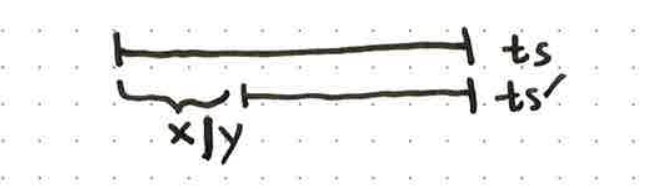
\includegraphics[width=180pt]{images/10-4.png}}
  % \caption{ CAPTION }
\end{figure}

\begin{lstlisting}
    -- parse px ts ++ parse py ts = parse (px <|> py) ts  \end{lstlisting}

Sometimes we want to extend \lstinline{<|>} to many input parsers.

\begin{lstlisting}
    choice :: [Parser a] -> Parser a
    choice pxs = foldr (<|>) empty pxs  \end{lstlisting}

We can define a combinator that appends the result of a parse onto others:

\begin{lstlisting}
    (<:>) :: Parser a -> Parser [a] -> Parser [a]
    px <:> pxs = (:) <s> px <*> pxs  \end{lstlisting}

To understand this, first recall that most parser combinators are left associative.

\begin{lstlisting}
    (:) <s> px <*> pxs
  =
    ((:) <s> px) <*> pxs

    -- check the types to see this is correct, recall:
    -- (<s>) :: (a -> b) -> f a -> f b
    -- (<*>) :: f (a -> b) -> f a -> f b  \end{lstlisting}

Now we're ready to define combinators that correspond to \lstinline{+} and \lstinline{*} from BNF.
\begin{itemize}
  \item $e+$ is written some e
  \item $e*$ is written many e
\end{itemize}

\begin{lstlisting}
    some :: Parser a -> Parser [a]
    some px = px <:> many px  \end{lstlisting}

this parses one \lstinline{px} and appends it to the result of many \lstinline{px}

\begin{lstlisting}
    many :: Parser a -> Parser [a]
    many px = some px <|> empty  \end{lstlisting}

\subsection{Monadic Parsing}

Sometimes we want the control flow a parser to depend on what was parsed. Suppose
we have \lstinline{px :: Parser a}, we can define a function \lstinline{f :: a -> Parser b}. The function
\lstinline{f} inspects the value \lstinline{x} which came from \lstinline{px} and produces a new parser accordingly.
The result should be a parser of time \lstinline{Parser b}.

\begin{lstlisting}
    instance Monad Parser where
      -- return :: a -> Parser a
      return :: pure -- from Applicative

      -- (>>=) :: Parser a -> (a -> Parser b) -> Parser b
      Parser px >>= f = Parser ( \ts ->
                      concat [parse  (f x) ts' | (x, ts') <- px ts])  \end{lstlisting}

\begin{figure}[H]
  \centering
  \fbox{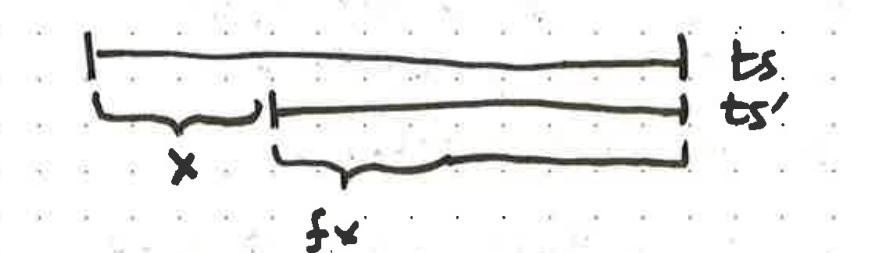
\includegraphics[width=180pt]{images/11-3.png}}
  % \caption{ CAPTION }
\end{figure}

To use this combinator we combine a parser with a function. The satify parser takes
in a function that is a predicate on \lstinline{Char}s and returns the parsed value if it
satisfies the predicate.

\begin{lstlisting}
    satisfy :: (Char -> Bool) -> Parser Char
    satisfy p = item >>= \t -> if p t
                                  then pure t
                                  else empty  \end{lstlisting}

This is perhaps the most useful combinator. Rather than the monadic definition, we can write
one directly:

\begin{lstlisting}
    satisfy :: (Char -> Bool) -> Parser Char
    satisfy p = Parser (\ts -> case ts of
                    []      -> []
                    (t:ts') -> [(t,ts') | p t])  \end{lstlisting}

We can now parse a single character as follows:

\begin{lstlisting}
    char :: Char -> Parser Char
    char c = satisfy (c ==)

    -- or char c = satisy (\c' -> c == c')  \end{lstlisting}

Example:

\begin{lstlisting}
    parse (char 'x') "xyz" = [('x',"yz")]
    parse (char 'a') "xyz" = []  \end{lstlisting}

%---------- see Lecture 12 - demonstration lecture. lhs file on blackboard.

\subsection{Chain for left-recursion}

The problem with ambiguous grammars that are left-recursive can be resolved with
Paull's algorithm.

\begin{lstlisting}
    <expr> ::= <number> | <expr> "+" <expr>  \end{lstlisting}

However, without applying Paull's algorithm, we have a nice data type:

\begin{lstlisting}
    data Expr = Num Int | Add Expr Expr  \end{lstlisting}

We can decide to use \lstinline{chainl1} to parse into this data structure from the original
grammar, assuming that $+$ is left associative. (\lstinline{chainr} exists if we want it to be
right associative). Essentially, we have this combinator:

\begin{lstlisting}
    chainl1 :: Parser a -> Parser (a->a->a) -> Parser a  \end{lstlisting}

This allows us to write a parser of the form:

\begin{lstlisting}
    expr :: Parser Expr
    expr = chainl1 number add

    add :: Parser (Expr -> Expr -> Expr)
    add = Add <s tok "+"  \end{lstlisting}

\section{Abstraction and Semantics}

\subsection{The Free Monad}

Suppose we are interested in giving a semantics to a language for addition. The
syntax for this language could look like \lstinline{x+y}. This corresponds
to a syntax tree:

\begin{figure}[H]
  \centering
  \fbox{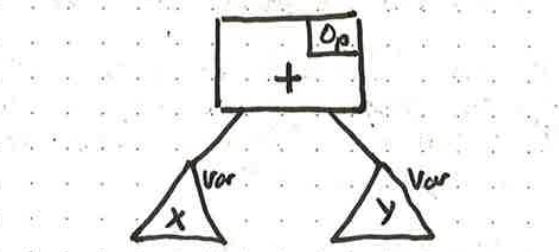
\includegraphics[width=180pt]{images/13-2.png}}
  % \caption{ CAPTION }
\end{figure}

Or for a more complex example, consider \lstinline{(x+y)+z}:

\begin{figure}[H]
  \centering
  \fbox{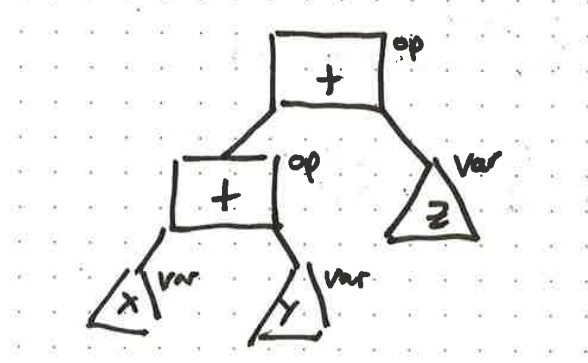
\includegraphics[width=180pt]{images/13-2-1.png}}
  % \caption{ CAPTION }
\end{figure}

We want to give the shape of \lstinline{+} nodes by using a signature functor:

\begin{lstlisting}
    data Add k = Add k k  \end{lstlisting}

In Haskell we can also write:

\begin{lstlisting}
    data Add k = k :+ k  \end{lstlisting}

The provision of variables is left to the Free Monad. The free monad \lstinline{Free f a} provides syntax
trees whose nodes are shaped by \lstinline{f}, and whose variables come from the type \lstinline{a}.

\begin{lstlisting}
    data Free f a = Var a
                  | Op (f (Free f a))  \end{lstlisting}

It is worth comparing this to the definition of \lstinline{Fix}:

\begin{lstlisting}
    data Fix f = In (f (Fix f))  \end{lstlisting}

The previous trees can be expressed with the following values of type \lstinline{Free Add String}.

\begin{lstlisting}
    Op (Add (Var "x") (Var "y"))

    Op (Add (Op (Add (Var "x") (Var "y")))(Var "z"))  \end{lstlisting}

To interpret these free trees, we work in two stages:

\begin{enumerate}
  \item We change the variables into values. \textit{(the Generator)}
  \item We evaluate the operations. \textit{(The Algerba)}
\end{enumerate}

In pictures, we do this to interpret a tree\footnote{The triangles on the second tree are an error.}:

\begin{figure}[H]
  \centering
  \fbox{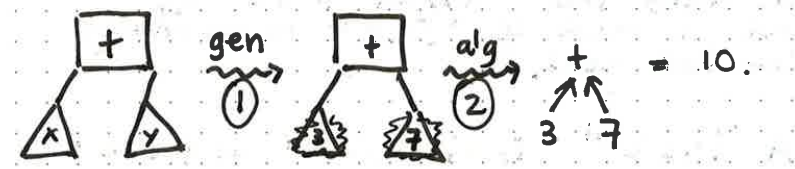
\includegraphics[width=300pt]{images/13-4.png}}
  % \caption{ CAPTION }
\end{figure}

\textit{(Stage 1)} The first stage involves replacing variables with their corresponding numbers. This
is achieved by defining \lstinline{Free f} to be a functor. This is only possible is \lstinline{f} is a
functor too.

\begin{lstlisting}
    instance Functor f => Functor (Free f) where
     -- fmap :: (a->b) -> Free f a -> Free f b
        fmap h (Var x) = Var (h x)
        fmap h (Op op) = Op (fmap (fmap h) op)

        -- note that op :: f (Free f a)  \end{lstlisting}

\begin{figure}[H]
  \centering
  \fbox{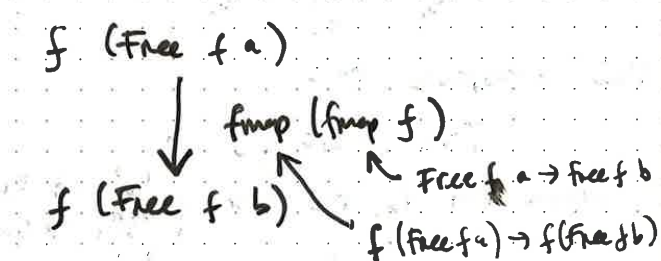
\includegraphics[width=180pt]{images/13-4-1.png}}
  % \caption{ CAPTION }
\end{figure}

\textit{(Stage 2)} The second stage extracts semantics by applying an algebra. This is a recursive function
defined as follows (We could use a \lstinline{cata}, but that is out of the scope of this lecture series).

\begin{lstlisting}
    extract :: Functor f => (f b -> b) -> Free f b -> b
    extract alg (Var x) = x
    extract alg (Op op) = alg (fmap (extract alg) op)

    -- x :: b, op :: f (Free f b)  \end{lstlisting}

Finally, we can combine these two stages to define an evaluation function:

\begin{lstlisting}
    eval :: Functor f => (f b -> b) (a -> b) -> Free f a -> b
    eval alg gen = extract alg . fmap gen

    -- fmap gen is stage 1, extract alg is stage 2  \end{lstlisting}

In pictures, we can represent an operation with a box, and a variable with a triangle,
and \lstinline{alg} will replace boxes, \lstinline{gen} will replace triangles. First we define an algebra for
a functor. Consider the \lstinline{Add} functor from before.

\begin{lstlisting}
    add :: Add Int -> Int
    add (x :+ y) = x + y  \end{lstlisting}

We also need a generator from the type of our variables. Variables are often given
as strings:

\begin{lstlisting}
    type Var = String  \end{lstlisting}

The Generator for addition is a function from \lstinline{Var} to \lstinline{Int}.

\begin{lstlisting}
    env :: Var -> Int
    env "x" = 3
    env "y" = 5
    env  $\_$   = 0  \end{lstlisting}

This is the environment for evaluation. Suppose we want to evaluate this tree:

\begin{figure}[H]
  \centering
  \fbox{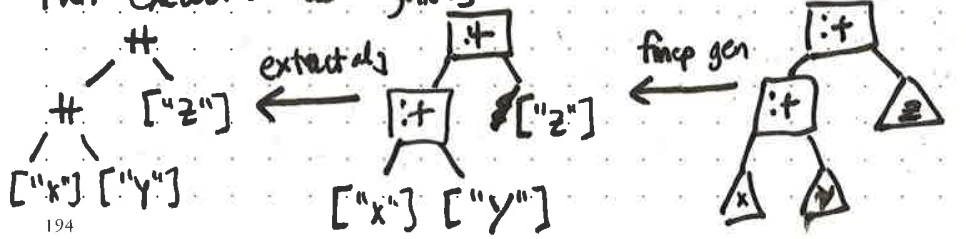
\includegraphics[width=300pt]{images/14-3-1.png}}
  % \caption{ CAPTION }
\end{figure}

This is an example of \lstinline{eval add env}. A second example is to collect all
variables in an expression as a list. To do this we provide a function \lstinline{Vars},
which is defined used \lstinline{eval}.

\begin{lstlisting}
    vars :: Free Add Var -> [Var]
    vars = eval alg gen
        where
            gen :: Var -> [Var]
            gen x = [x]

            alg :: Add [Var] -> [Var]
            alg (xs :+ ys) = xs ++ ys  \end{lstlisting}

This executes as follows:

\begin{figure}[H]
  \centering
  \fbox{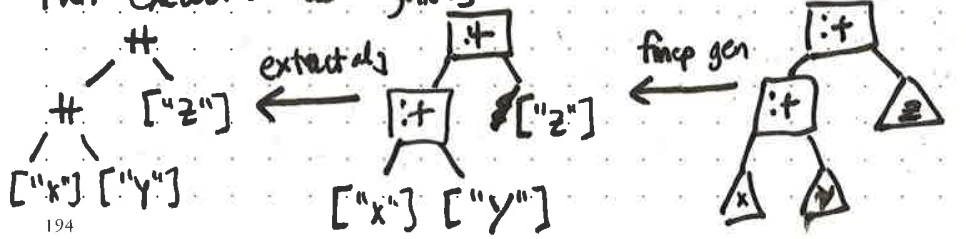
\includegraphics[width=300pt]{images/14-3-1.png}}
  % \caption{ CAPTION }
\end{figure}

Suppose we want to add an operation to our language, that performs division.

\begin{lstlisting}
    data _Div_ k = _Div_ k k  \end{lstlisting}

If we want to provide a semantics that collects all the variables, we must provide
an algebra.

\begin{lstlisting}
    divVars :: _Div_ [Var] -> [Var]
    divVars (_Div_ xs ys) = xs ++ ys  \end{lstlisting}

If we want a language with both addition and division, we need to take the coproduct of
\lstinline{_Add_} and \lstinline{_Div_}. This means expressions of the form \lstinline{_Add_ :+: _Div_}. For example, we can work with \lstinline{_Div_} alone:

\begin{lstlisting}
    evalDiv :: Free Div Var -> [Var]
    evalDiv = eval alg gen where
        gen :: Var -> [Var]
        gen x = [x]

        alg :: _Div_ [Var] -> [Var]
        alg (_Div_ xs ys) = xs ++ ys  \end{lstlisting}

Dealing with both \lstinline{_Add_} and \lstinline{_Div_} at once requires this:

\begin{lstlisting}
    vars :: Free (_Add_ :+: _Div_) Var -> [Var]
    vars = eval alg gen where
        gen x = [x]

        alg :: (_Add_ :+: _Div_) [Var] -> [Var]
        alg (L (_Add_ xs ys)) = xs ++ ys
        alg (R (_Div_ xs ys)) = xs ++ ys  \end{lstlisting}

When we try to evaluate this language, naively, we encounter a problem.

\begin{lstlisting}
    expr :: Free (_Add_ :+: _Div_) Var -> Double
    expr = eval alg gen where
        gen :: Var -> Double
        gen = env -- this function magically knows how to assign
                     values to variables

        alg :: _Add_ :+: _Div_ Double -> Double
        alg (L (_Add_ x y)) = x + y
        alg (R (_Div_ x y)) = x / y  \end{lstlisting}

The sad truth is that this function is broken. To see why, consider
\lstinline{alg (R (_Div_ x 0))}. This will fail! To fix this problem, we must be upfront about the
fact that an error can happen. The basic way to do this is to interpret into a
\lstinline{Maybe} datatype.

\begin{lstlisting}
    expr :: Free (_Add_ :+: _Div_) Var -> Maybe Double
    expr = eval alg gen where
        gen = env

        alg (L (_Add_ x y)) = mAdd  -- {note x :: Maybe Double}
        alg (R (_Div_ x y)) = mDiv  \end{lstlisting}

We must now define \lstinline{mAdd} and \lstinline{mDiv}, with division we are sensitive to zero:

\begin{lstlisting}
    mAdd :: Maybe Double -> Maybe Double -> Maybe Double
    mAdd (Just x) (Just y) = Just (x + y)
    mAdd mx my             = Nothing

    mDiv :: Maybe Double -> Maybe Double -> Maybe Double
    mDiv (Just x) (Just 0) = Nothing
    mDiv (Just x) (Just y) = Just (x / y)
    mDiv mx my             = Nothing  \end{lstlisting}

\subsection{Failure}

We need to create syntax for failure:

\begin{lstlisting}
    data _Fail_ k = _Fail_

    instance Functor _Fail_ where
        fmap f _Fail_ = _Fail_  \end{lstlisting}

The functor instance shows us that computations can not follow a fail. If we deal
with division alone, we have this:

\begin{lstlisting}
    evalFail :: Free _Div_ Double -> Free _Fail_ Double
    evalFail = eval alg gen
        where
            gen :: Double -> Free _Fail_ Double
            gen x = Var x

            alg :: _Div_ (Free _Fail_ Double) -> Free _Fail_ Double
            alg (_Div_ (Var x) (Var 0)) = Op _Fail_
            alg (_Div_ (Var x) (Var y)) = Var (x / y)
            alg (_Div_    tl      tr )  = Op _Fail_  \end{lstlisting}

\subsection{Substitution}

Substitution in a language is a very useful feature. For example, consider \lstinline{x+7}. We can
evaluate this into a new syntax tree when we have a notion of substitution, where we might bind
\lstinline{x} to another expression rather than just a constant, like \lstinline{x $\rightarrow$ x+5},
then we expect the above to become \lstinline{(4+5)+7}. We can depict this by the following trees.

\begin{figure}[H]
\centering
\begin{subfigure}{.5\textwidth}
  \centering
  \fbox{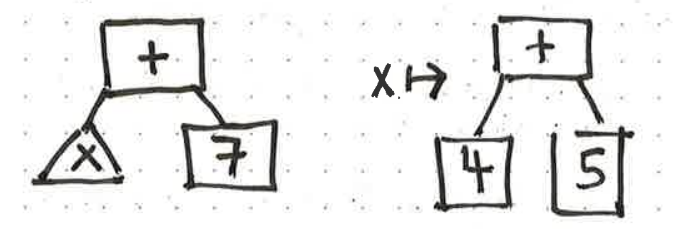
\includegraphics[width=180pt]{images/16-1.png}}
\end{subfigure}%
\begin{subfigure}{.5\textwidth}
  \centering
  \fbox{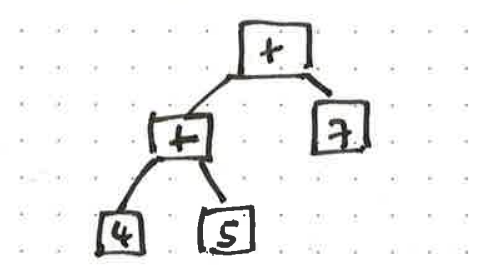
\includegraphics[width=180pt]{images/16-2.png}}

\end{subfigure}
\end{figure}

We will define substitution using code. Usuaully an expression \lstinline{e} with a variable \lstinline{x}
is substituted with \lstinline{e'} with the following syntax:

\begin{lstlisting}
    e [x $\rightarrow$ e']  \end{lstlisting}

where \lstinline{e} corresonds to \lstinline{x+7}, and \lstinline{e'} is \lstinline{4+5}. Sometimes we write:

\begin{lstlisting}
    e [x $\backslash$ 4+5]
    -- or
    e [4+5 / x]  \end{lstlisting}

For our purposes, a syntax tree is given by a datatype \lstinline{Free f a}, where \lstinline{f} is the shape of the syantx,
and \lstinline{a} is the type of the variables, substitution is defined by \lstinline{(>>=)} as follows:

\begin{lstlisting}
    (>>=) :: Free f a -> (a -> Free f b) -> Free f b
    Var x >>= f  =  f x
    Op op >>= f  =  Op (fmap (>>= f) op)  \end{lstlisting}

\subsection{Non-Determinism}

A non-deterministic computation is one that provides the choice between two different computations.
For example, \lstinline{p $\Box$ q} is the program that gives answers from p or q.

\begin{figure}[H]
  \centering
  \fbox{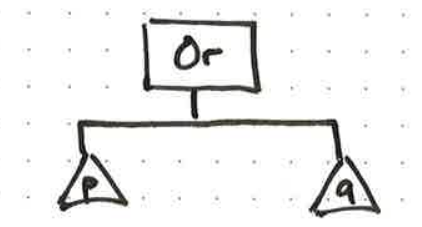
\includegraphics[width=180pt]{images/16-3.png}}
  % \caption{ CAPTION }
\end{figure}

Here we use \lstinline{Or} to represent $\Box$.

\begin{figure}[H]
  \centering
  \fbox{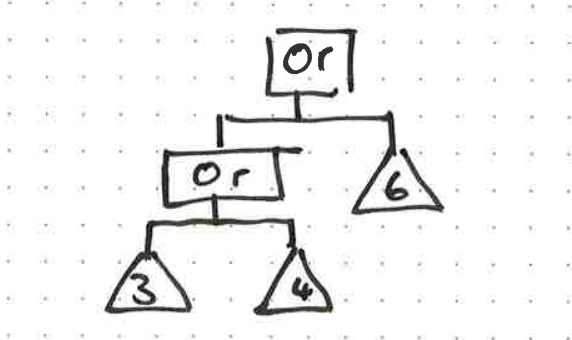
\includegraphics[width=130pt]{images/16-3-1.png}}
  % \caption{ CAPTION }
\end{figure}

One interprets this tree as follows:

\begin{figure}[H]
  \centering
  \fbox{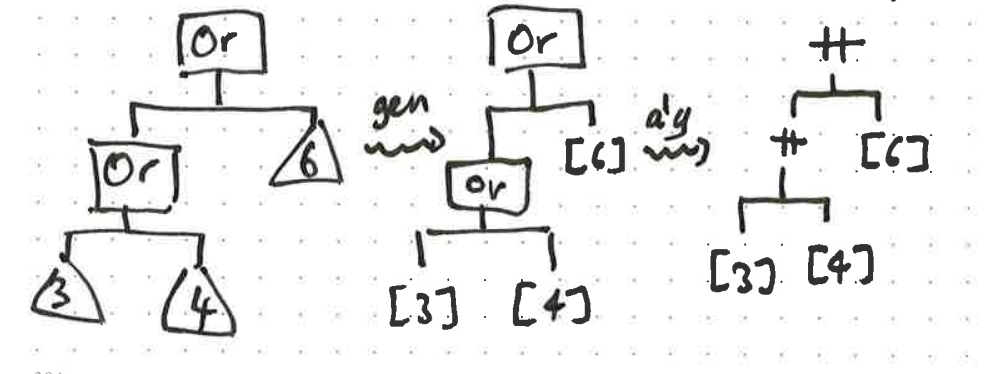
\includegraphics[width=260pt]{images/16-3-2.png}}
  % \caption{ CAPTION }
\end{figure}

In terms of code, we first need to express syntax, we must also create a functor instance.
With this in place, we can define an evaluation function:

\begin{lstlisting}
    data Or k = Or k k

    instance Functor Or where
        fmap f (Or x y) = Or (f x) (f y)

    list :: Free Or a -> [a]
    list = eval alg gen where
        gen :: a -> [a]
        gen :: x =  [x]

        alg :: Or [a] -> [a]
        alg (Or xs ys) = xs ++ ys  \end{lstlisting}

Another interpretation of these trees is to simply return the first result. We can define the semantics
using \lstinline{once}.

\begin{lstlisting}
    once :: Free Or a -> Maybe a
    once = eval alg gen where
        gen :: a -> Maybe a
        gen x = Just x

        alg :: Or (Maybe a) -> Maybe a
        alg (Or Nothing y)  = y
        alg (Or (Just x) y) = Just x  \end{lstlisting}

This works, but we want a way of signalling that there was no solution. For this, we
will make use of \lstinline{Fail}. Nondeterminism is the syntax provided by the following
synonym.

\begin{lstlisting}
    type Nondet a = (Fail :+: Or) a  \end{lstlisting}

Trees of type \lstinline{Free Nondet a} have this shape:

\begin{figure}[H]
  \centering
  \fbox{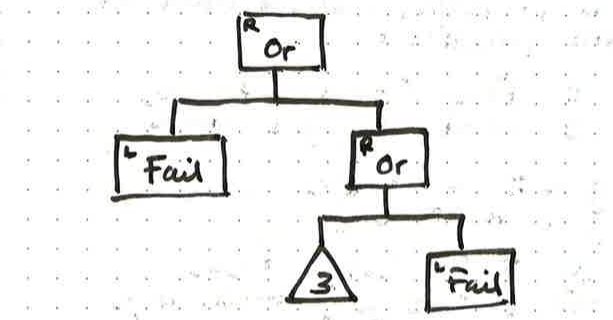
\includegraphics[width=180pt]{images/17-2.png}}
  % \caption{ CAPTION }
\end{figure}

As before, we give semantics to \lstinline{Nondet} languages by providing a generator
and an algebra.

\begin{lstlisting}
    list :: Free Nondet a -> [a]
    list = eval alg gen where
        gen :: a -> [a]
        gen x = [a]

        alg :: Nondet [a] -> [a]
        alg (L Fail)     = []
        alg (R (Or x y)) = x ++ y  \end{lstlisting}

The semantics for \lstinline{once} is similar.
% TODO define once

\subsection{Alternation}

An alternative way to do \lstinline{Or} is to model a pair of \lstinline{k} values
as a function from \lstinline{Bool}. For this, we define the following:

\begin{lstlisting}
    data Alt k = Alt (Bool -> k)

    instance Functor Alt where
        fmap :: (a -> b) -> Alt a -> Alt b
        fmap f (Alt k) = Alt (f . k)  \end{lstlisting}

The idea is that we parse \lstinline{True} when we want the first child, and \lstinline{False}
for the second child. Now we can give different semantics for nondeterminism.

\begin{lstlisting}
    type Nondet' a = (Fail :+: Alt) a

    list :: Free Nondet' a -> [a]
    list = eval alg gen where
        gen :: a -> [a]
        gen x = [x]

        alg :: Nondet' [a] -> [a]
        alg (L Fail)    = []
        alg (R (Alt k)) = k True ++ k False

        -- k :: Bool -> [a]  \end{lstlisting}

This demonstrates that the parameter to a syntax functor sometimes has the form of a
function, i.e. \lstinline{Bool -> k}.

\subsection{State}

A stateful computation can be modelled by having two operations, \lstinline{Get}
and \lstinline{Put}.

\begin{lstlisting}
    data State s k = Put s k
                   | Get (s -> k)  \end{lstlisting}

The intuition is that \lstinline{Put s k} will put the value \lstinline{s} into the
state before continuing with the computation \lstinline{k}. The \lstinline{Get f}
operation will only continue when \lstinline{f :: s -> k} is given a variable of type
\lstinline{s}. The semantic domain for \lstinline{State} is a function of type:

\begin{lstlisting}
    s -> (a,s)  \end{lstlisting}

This is a carrier for stateful computations.

\begin{lstlisting}
    evalState :: Free (State s) a -> (s -> (a,s))
    evalState = eval alg gen where
        gen :: a -> (s -> (a,s))
        gen x s = (a,s)
        -- or equivalently gen x = \s -> (x,s)

        alg :: State s (s -> (a,s)) -> (s -> (a,s))
        alg (Put s' k) = \s -> k s'
        alg (Get k)    = \s -> k s s
        -- in k s s, the first s is the state that generates programs,
           and the second is the state parsed on to future programs.  \end{lstlisting}

This function carries on computations generated by \lstinline{k} when supplied with
the new state \lstinline{s}.

\subsection{Diagrams of operations}

We have already seen many diagrams, here are some conventions:

\begin{table}[htp]
\begin{tabular}{lp{0.67\textwidth}}
  \raisebox{-0.5\totalheight}{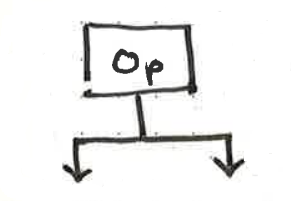
\includegraphics[width=60pt]{images/18-1.png}}
  & \tabitem Operations are written in boxes, and the arrows emerging
    below represent different $k$ values. \\
  \raisebox{-0.5\totalheight}{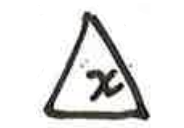
\includegraphics[width=40pt]{images/18-1-1.png}}
  & \tabitem Trianglular leaves represent variables. \\
  \raisebox{-0.5\totalheight}{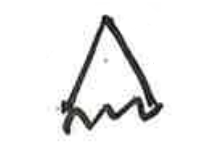
\includegraphics[width=40pt]{images/18-1-2.png}}
  & \tabitem We will often represent an arbitrary subtree with this.
\end{tabular}
\end{table}

To represent nondeterminism and alternation, we have these diagrams:

\begin{lstlisting}
    data Or  k = Or k k
    data Alt k = Alt (Bool -> k)  \end{lstlisting}

\begin{figure}[H]
  \centering
  \fbox{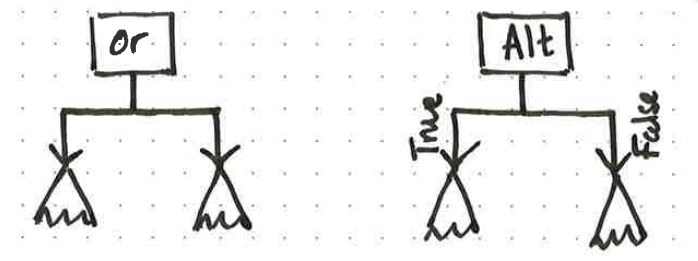
\includegraphics[width=180pt]{images/18-2.png}}
  % \caption{ CAPTION }
\end{figure}

We can imagine that \lstinline{State s = Put s :+: Get s}:

\begin{lstlisting}
    data Put s k = Put s k
    data get s k = Get (s -> k)  \end{lstlisting}

To draw the operation \lstinline{Put}, we have the following:

\begin{figure}[H]
  \centering
  \fbox{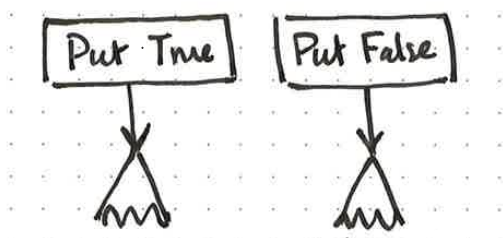
\includegraphics[width=180pt]{images/18-2-1.png}}
  % \caption{ CAPTION }
\end{figure}

These examples are of \lstinline{Free (Put Bool) a} syntax trees: Since
\lstinline{s = Bool} we can only construct these two \lstinline{Put} nodes.
We cab parameterise \lstinline{s} different, so if we had \lstinline{s = Int},
we would have a huge (infinite) number of nodes:
\begin{figure}[H]
  \centering
  \fbox{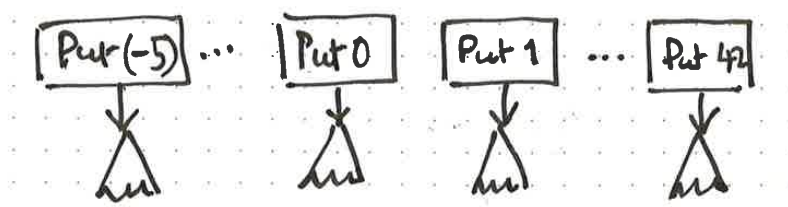
\includegraphics[width=180pt]{images/18-3.png}}
  %\caption{}
\end{figure}

The \lstinline{Get} nodes are a generalisation of \lstinline{Alt}. If we consider
trees of the form \lstinline{Free (Get Bool) a} then this is as follows:

\begin{figure}[H]
  \centering
  \fbox{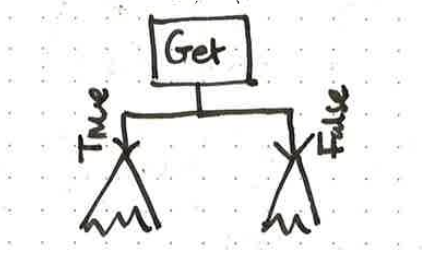
\includegraphics[width=180pt]{images/18-3-1.png}}
  %\caption{A \lstinline{Free (Get Bool) a} tree.}
\end{figure}

However, with \lstinline{s = Int}, we have \lstinline{Free (Get Int) a}:

\begin{figure}[H]
  \centering
  \fbox{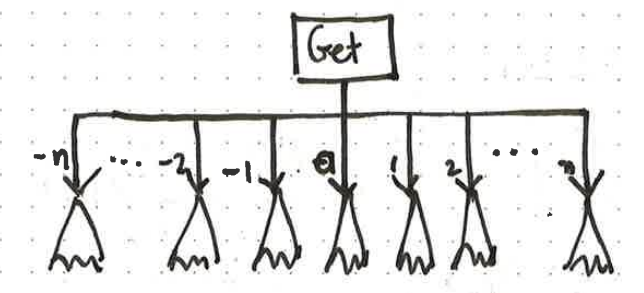
\includegraphics[width=180pt]{images/18-3-2.png}}
  % \caption{ CAPTION }
\end{figure}

Note that \lstinline{Alt} and \lstinline{Get Bool} are not syntactically very
similar; they share the same structure but their differences are exhibited when
we provide different algebras. Another thing we can do is compose trees together:

\begin{figure}[H]
  \centering
  \fbox{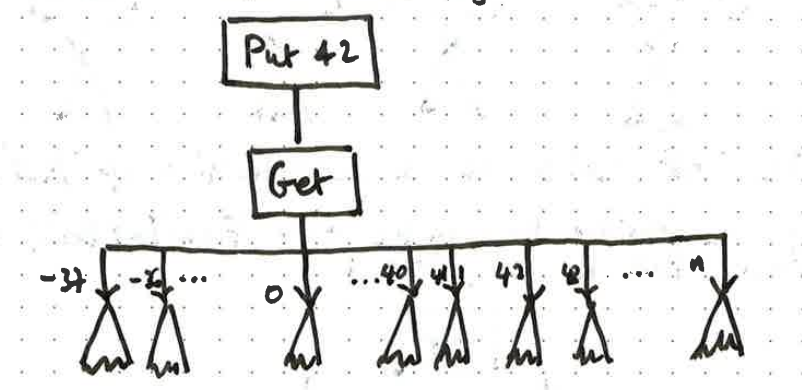
\includegraphics[width=180pt]{images/18-4.png}}
  % \caption{ CAPTION }
\end{figure}

When we gave the algebra for \lstinline{State s} when the carrier was \lstinline{s -> (a,s)},
we were storing the state \lstinline{s} in output, and reacting as \lstinline{s}
as input. Consider \lstinline{s = Bool}:

\begin{figure}[H]
  \centering
  \fbox{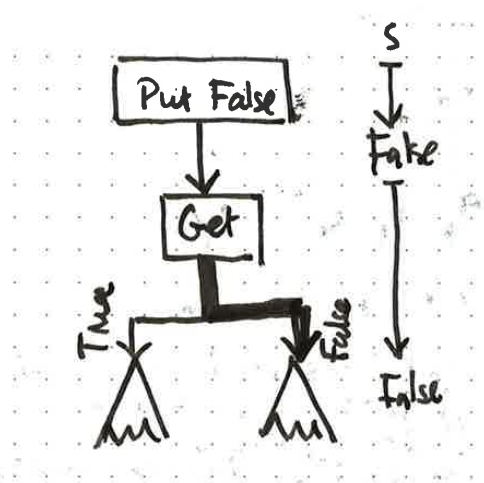
\includegraphics[width=120pt]{images/18-4-1.png}}
  % \caption{ CAPTION }
\end{figure}

Note that here we have used \lstinline{False} to choose which child to use, and
we also passed \lstinline{False} on to the next stage.

\begin{lstlisting}
    alg (Get k) = \s -> k s s

    -- The k in 'Get k' is represented by the children in the diagram.
    -- The first s in 'k s s' is selecting the child.
    -- The second s is passing the s onwards.  \end{lstlisting}

These syntax trees all correspond to values of type \lstinline{Free (State s) a}.
They can be cumbersome to work with because we must wrap everything in \lstinline{Op}.

\begin{lstlisting}
    Op (Put False (Op (Get (\s -> $\ldots$))))  \end{lstlisting}

We can avoid this by introducing smart constructors for \lstinline{Put} and
\lstinline{Get}:

\begin{lstlisting}
    put :: s -> Free (State s) ()
    put s = op (Put s (Var ()))

    get :: Free (State s) s
    get = Op (Get (\s -> Var s))  \end{lstlisting}

And with these tools, we can simply substitute

\begin{lstlisting}
    put False >> get  \end{lstlisting}

and this produces the same tree as above.




\end{document}
